\documentclass[11pt]{article}
\usepackage{amssymb}
\usepackage{amsthm}
\usepackage[fleqn]{amsmath}
\usepackage{listings}
\usepackage{color}
\usepackage{graphicx}
\usepackage{subcaption}
\usepackage[margin=1.0in]{geometry}

\lstdefinestyle{matlab-style}{
language=Matlab,
basicstyle=\scriptsize\ttfamily,
tabsize=2,
rulecolor=,
language=matlab,
basicstyle=\scriptsize,
aboveskip={1.5\baselineskip},
columns=fullflexible,
showstringspaces=false,
extendedchars=true,
breaklines=true,
prebreak = \raisebox{0ex}[0ex][0ex]{\ensuremath{\hookleftarrow}},
frame=single,
showtabs=false,
showspaces=false,
showstringspaces=false,
identifierstyle=\ttfamily,
keywordstyle=\color[rgb]{0,0,1},
commentstyle=\color[rgb]{0.133,0.545,0.133},
stringstyle=\color[rgb]{0.627,0.126,0.941},
keepspaces=true,
numbers=left,
numbersep=5pt,
numberstyle=\tiny\color[rgb]{0.5,0.5,0.5},
stepnumber=1
}

\newcommand{\bs}[1] {\boldsymbol{#1}}

\title{Mandating fun on a tilt-o-whirl : MANE 6963 - Project 3}
\author{ID: 2168}
\date{}

\begin{document}

\maketitle

\section{Executive summary}

In this report, we investigate the optimal design of a
tilt-o-whirl amusement ride, where riders' cars spin
independently about a platform, while also spinning
about a central platform. Our objective is to maximize
the standard deviation of the angular velocity of each
car on the platform, which is thought to increase
the unpredictability and thus fun of the ride.
Figure \ref{fig:ride} depicts various variables
associated with the tilt-o-whirl ride design.
The physical meaning of these variables is described
in Table \ref{table:variables}. Using these variables,
the objective function we would like to maximize is
written as $f = \sigma(d \phi / d t)$, where $\sigma$
denote the standard deviation.

\begin{figure}[hbt!]
\centering
\begin{subfigure}{.25\textwidth}
\centering
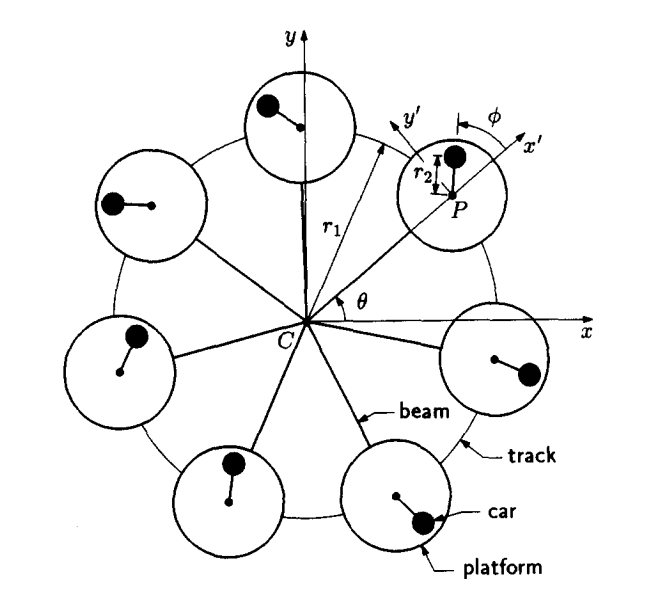
\includegraphics[width=.99\linewidth]{ride1}
\end{subfigure}%
\begin{subfigure}{.25\textwidth}
\centering
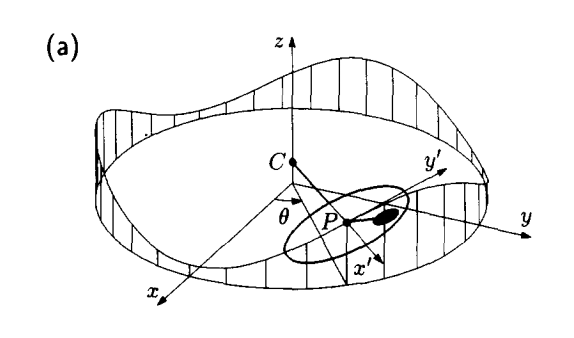
\includegraphics[width=.99\linewidth]{ride2}
\end{subfigure}%
\begin{subfigure}{.25\textwidth}
\centering
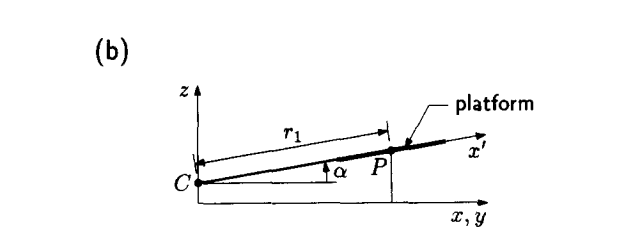
\includegraphics[width=.99\linewidth]{ride3}
\end{subfigure}%
\begin{subfigure}{.25\textwidth}
\centering
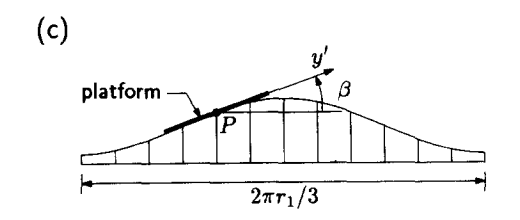
\includegraphics[width=.99\linewidth]{ride4}
\end{subfigure}
\caption{Tilt-o-whirl ride diagrams \cite{chaos}}
\label{fig:ride}
\end{figure}

\begin{table}[hbt!]
\centering
\begin{tabular}{c | c}
parameter name & description \\ \hline \hline
$\theta$ & angle defining platform location \\ \hline
$\omega$ & angular velocity of the base \\ \hline
$\alpha$ & angle to describe tilt of car platform \\ \hline
$\beta$ & angle to describe tilt of car platform \\ \hline
$r_1$ & base arm radius \\ \hline
$r_2$ & radius to car pivot point \\ \hline
$\phi$ & angle defining car location \\ \hline
$\frac{d \phi}{d t}$ & car angular velocity \\ \hline
\end{tabular}
\caption{Parameters used to describe tilt-o-whirl motion}
\label{table:variables}
\end{table}

The remainder of this report is structured as follows.
First, we provide a summary of the analysis method
used to evaluate the standard deviation of the car's
angular velocity, which involves the numerical solution
of a chaotic dynamical system. We then verify the
solution numerical analysis by comparison to known
results. Next, we discuss the optimization methods used
to achieve the optimization goal. Due to the chaotic
nature of the dynamical ODE, we approximate the actual
objective function with a surrogate model.
The construction and verification of this surrogate
model is discussed. Next, the optimization problem
is stated and its implementation using the developed
surrogate model is discussed. Finally, results are
presented and we conclude that our tilt-o-whirl design
is sufficiently fun based on comparison to nominal
values. All code developed for this project is listed
in the appendix.

\section{Analysis methods}

\subsection{Model}

As mentioned, the motion of the car platform can be
predicted via a chaotic, dynamical ODE. Following
Kautz and Huggard \cite{chaos}, this ODE can be
expressed as:
%
\begin{equation}
\frac{d^2 \phi}{d \tau^2} +
(\gamma / Q_0) \frac{d \phi} {d \tau} +
(\epsilon - \gamma^2 \alpha) \sin \phi +
(\gamma^2 \beta) \cos \phi,
\end{equation}
%
where $\tau = 3 \omega t$ is a non-dimensional time
parameter, $\gamma = \frac{1}{3 \omega} \sqrt{g/r_2}$
and $\epsilon = \frac{r_1}{9 r_2}$ are dimensionless
parameters, and $Q_0$ is a parameter chosen to be fixed
at the value $20$. This second order ODE can be written
as a system of first order ODEs by introducing the
variables $y_1 = \frac{d \phi}{d \tau}$, $y_2 = \phi$.
The system of ODEs is written as:
%
\begin{equation}
\frac{d}{d \tau}
\begin{bmatrix}
y_1\\
y_2
\end{bmatrix}
=
\begin{bmatrix}
F(y_1, y_2) \\
y_1
\end{bmatrix},
\end{equation}
%
where
%
\begin{equation}
F(y_1, y_2) =
(\gamma / Q_0) y_1 +
(\epsilon - \gamma^2 \alpha) \sin (y_2) +
\gamma^2 \beta \cos(y_2),
\end{equation}

Using the time-dependent solution
$y_1 = \frac{d \phi} {d \tau}$,
the standard deviation objective function can be
computed as:
%
\begin{equation}
f = 3 \omega
\sqrt{ \frac{1}{T} \int_0^T (y_1 - \bar{y}_1)^2 \text{d} \tau},
\label{eq:obj}
\end{equation}
%
where $\bar{y}_1 = \frac{1}{T} \int_0^T y_1 \text{d} \tau$,
and $T$ is the final non-dimensional integration time.
Finally, we note that the parameter $\alpha$ can be
expressed as $\alpha = \alpha_0 - \alpha_1 \cos \tau$,
where $\alpha_0$ is an angle offset coefficient
and $\alpha_1$ is associated with the incline angle.

\subsection{Implementation and verification}

The ODE driving function $F$ is implemented in the
code \textsc{F.m}, and the computation of the objective
function is implemented by \textsc{Obj.m}. To verify
the analysis code, we choose the nominal parameter
values $a^n_0 = 0.036$ rad, $a^n_1 = 0.058$ rad,
$r^n_1 = 4.3$ m, $r^n_2 = 0.8$ m, and
$\omega^n = 6.25 \frac{2 \pi}{60}$ rad s$^{-1}$.
Additionally, we choose
a final non-dimensional integration of $T = 2000$.
Note on line 18 of \textsc{Obj.m}, we determine initial
conditions for the ODE solve by performing a 'spin-up'
solve, where the ODE system is solved with zero initial
conditions over $5$ percent of the total integration time.
The Matlab routine \textsc{ode45} is utilized to solve
the ODE system.

\begin{figure}[hbt!]
\centering
\begin{subfigure}{.5\textwidth}
\centering
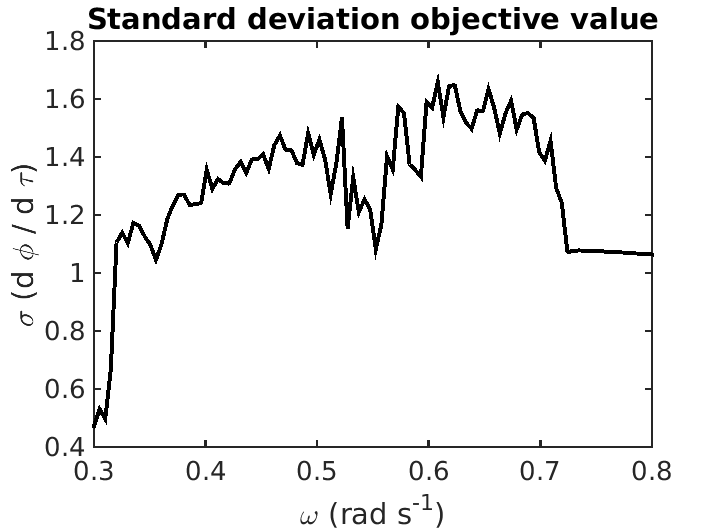
\includegraphics[width=.99\linewidth]{verify}
\end{subfigure}%
\begin{subfigure}{.5\textwidth}
\centering
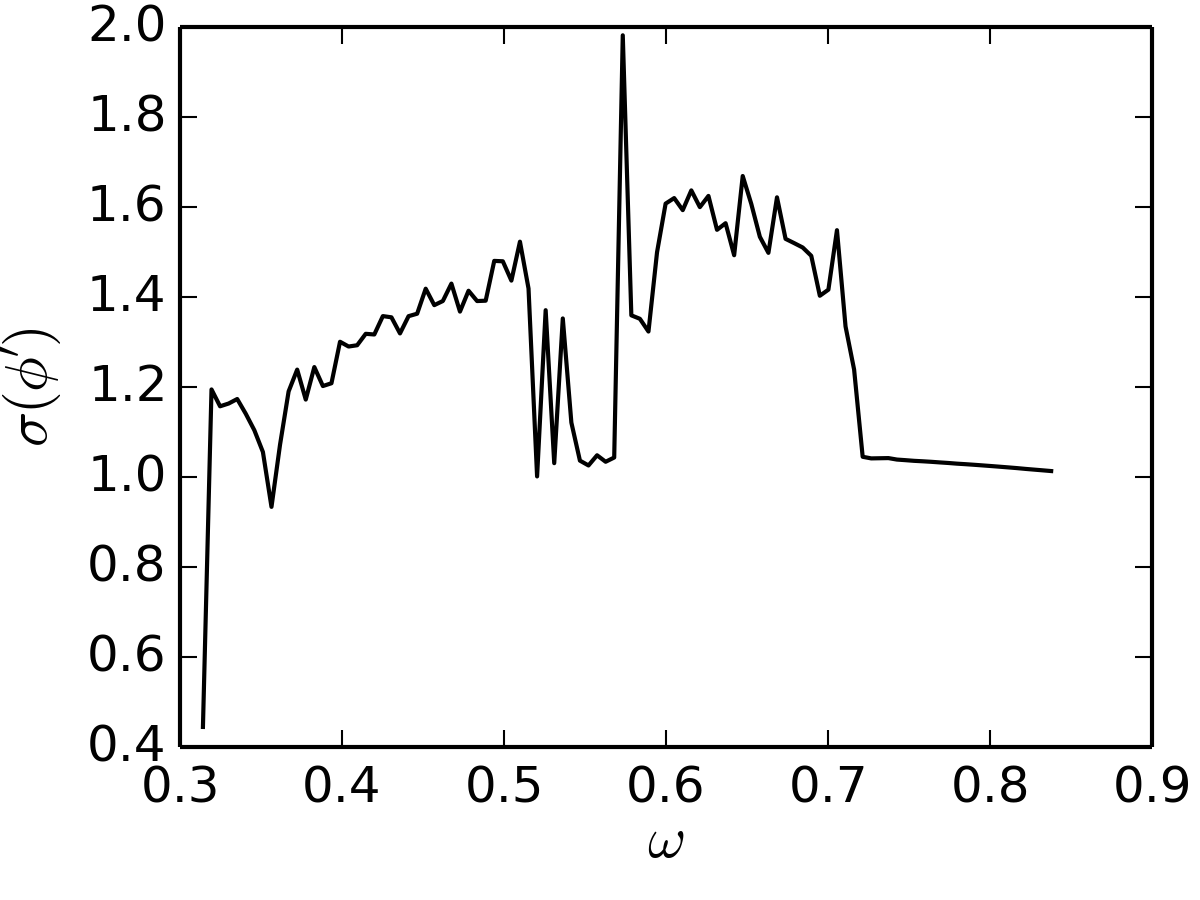
\includegraphics[width=.99\linewidth]{compare}
\end{subfigure}
\caption{Objective function evaluated at nominal
parameters versus $\omega$ using the developed code (left)
and a known working analysis code (right).}
\label{fig:verify}
\end{figure}

Figure \ref{fig:verify} shows results
obtained from the analysis routines implemented for this
project as compared to a known working analysis code.
The results agree qualitatively and quantitatively
and lead us to believe that the analysis code has
been implemented correctly. Additionally, we performed
the ODE solve to the final time $T$ using
$\omega \ll 1$ and $\omega \gg 1$. We observed that,
when $\omega \ll 1$, the solution $\phi$ exhibits
stable periodic behavior time, and when $\omega \gg 1$,
the solution $\phi$ exhibits chaotic unpredictable
behavior throughout its time evolution. This agrees
with the conclusions of \cite{chaos}.

\section{Optimization methods}

To achieve a fun tilt-o-whirl design, we choose the
following parameter vector $\bs{p} \in \mathbb{R}^3$ such that
%
\begin{equation}
\bs{p} = [ \omega,  r_2,  \alpha_1 ]^T,
\end{equation}
%
and we fix the variables $r_1 = r_1^n$
and $\alpha_0 = \alpha_0^n$. Further, we are interested
in the bounded design space defined by the bounds:
%
\begin{equation}
\begin{aligned}
3 \; \text{rpm} & \leq && \omega \frac{2 \pi}{60} &&\leq 8 \; \text{rpm} \\
0.1 \; \text{m} & \leq && r_2 &&\leq 1.5 \; \text{m} \\
0 \; \text{rad} & \leq && \alpha_1 &&\leq 0.3 \; \text{rad}
\label{eq:bounds}
\end{aligned}
\end{equation}
%
Presumably the upper bounds are set so that we don't
break children's necks.

\subsection{Surrogate model}

Due to the chaotic nature of the ODE system that is embedded in
the objective function and the fact that the objective function
is relatively expensive to compute directly, we construct a
surrogate model to approximate the objective function. We begin
this construction by randomly selecting $N_s = 100$ design sample
locations in the domain defined by the bounds \eqref{eq:bounds}.
This sampling is achieved with Latin Hypercube Sampling (LHS)
on line 32 of \textsc{Surrogate.m}. Figure \ref{fig:lhs}
illustrates one potential sampling of the design space using
LHS.

\begin{figure}[hbt!]
\centering
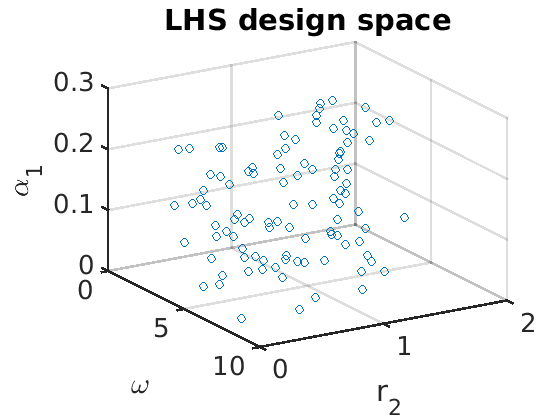
\includegraphics[width=.5\linewidth]{designspace}
\caption{Example design space sampling with LHS}
\label{fig:lhs}
\end{figure}

Next, we determine the hyper-parameters for our surrogate
model using the \textsc{GPML} library. These hyper-parameters
are the output of the method \textsc{Surrogate.m}. To `train'
the surrogate model to select the hyper-parameters, we
choose a Gaussian likelihood function as seen on line
45 of \textsc{Surrogate.m}, and a Mat\'{e}rn covariance
function as seen on line 41 of \textsc{Surrogate.m}.
Finally, in the training of our surrogate model, we allow
for some noise in the data by selecting the parameter
$s_n = 0.025$, as seen on line 44 of \textsc{Surrogate.m}
Once the hyper-parameters are found, a surrogate Gaussian
process model $\tilde{f}$ is fully defined that
approximates the objective function $f$. The Gaussian
process surrogate is sampled using the implemented
routine \textsc{OptObj.m}.

\subsection{Surrogate model verification}

To verify the construction of the surrogate model,
we sample the surrogate model evaluated at the nominal
variable values while parameter $\omega$. Figure
\ref{fig:surrogate} shows a comparison of the surrogate
objective value $\tilde{f}$ versus the analysis objective
value $f$ as the parameter $\omega$ varies.

\begin{figure}[hbt!]
\centering
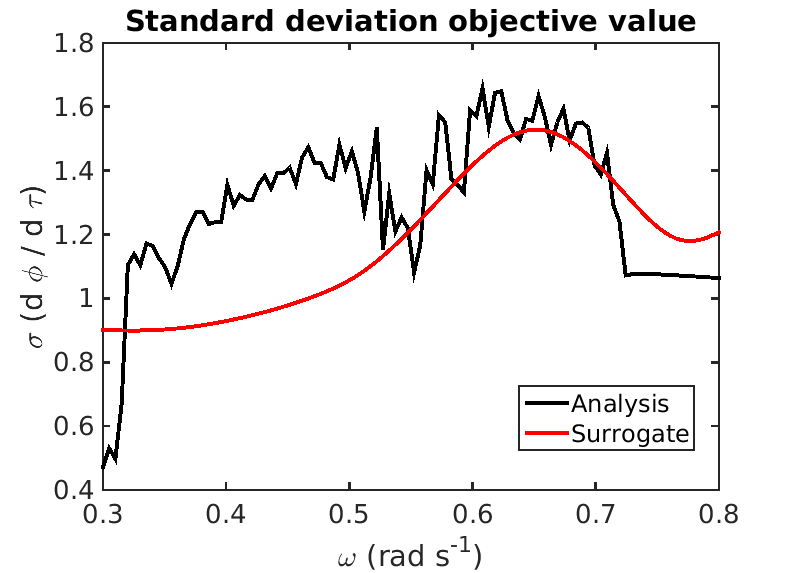
\includegraphics[width=.5\linewidth]{Verify2}
\caption{Surrogate model sampling with nominal values}
\label{fig:surrogate}
\end{figure}

\subsection{Optimization problem statement}

Given the surrogate Gaussian process, the optimization
problem statement becomes:
\begin{equation}
\begin{aligned}
& \underset{\bs{p}}{\text{minimize}}
& & \tilde{f}(\bs{p}) \\
& \text{subject to}
& & 3 \; \text{rpm} \leq p_1 \frac{2 \pi}{60} \leq \; 8 \text{rpm}, \\
&&& 0.1 \; \text{m} \leq p_2 \leq 1.5 \; \text{rpm}, \\
&&& 0 \; \text{rad} \leq p_3 \leq 0.3 \; \text{rad}\\
\end{aligned}
\end{equation}

\section{Results}

The construction of the surrogate model and the optimization
problem is encapsulated entirely in the script \textsc{Driver.m}.
We utilize Matlab's \textsc{fmincon} routine with default tolerances
to perform gradient-based optimization on the surrogate objective
function. The initial guess for the optimization routine is given
by the nominal design parameters. The convergence history of the
optimization routine is shown below:

{ \scriptsize
\begin{verbatim}
 Norm of First-order
 Iter F-count            f(x) Feasibility  Steplength        step  optimality
    0       4   -1.488281e+00   0.000e+00                           1.364e+01
    1       8   -2.126049e+00   0.000e+00   1.000e+00   4.781e-01   1.013e+01
    2      14   -2.175085e+00   0.000e+00   4.900e-01   3.790e-01   6.000e+00
    3      18   -2.732151e+00   0.000e+00   1.000e+00   4.389e-01   5.211e+00
    4      22   -4.702722e+00   2.776e-17   1.000e+00   5.857e-01   7.417e+00
    5      28   -4.731514e+00   1.388e-17   4.900e-01   7.872e-02   4.500e+00
    6      39   -4.812858e+00   0.000e+00   8.235e-02   8.437e-02   2.863e+00
    7      47   -4.816365e+00   0.000e+00   2.401e-01   3.087e-02   3.659e+00
    8      53   -4.822389e+00   0.000e+00   4.900e-01   6.119e-02   2.798e+00
    9      59   -4.894551e+00   0.000e+00   4.900e-01   5.556e-02   3.447e+00
   10      63   -4.928094e+00   0.000e+00   1.000e+00   2.138e-02   7.479e-01
   11      67   -4.931250e+00   0.000e+00   1.000e+00   4.901e-03   4.142e-01
   12      71   -4.932860e+00   0.000e+00   1.000e+00   7.100e-03   1.354e-01
   13      75   -4.932945e+00   0.000e+00   1.000e+00   1.270e-03   3.173e-02
   14      79   -4.932950e+00   0.000e+00   1.000e+00   2.553e-04   1.613e-03
   15      83   -4.932950e+00   0.000e+00   1.000e+00   1.574e-05   4.258e-04
   16      87   -4.932950e+00   0.000e+00   1.000e+00   3.167e-06   2.909e-05
   17      91   -4.932950e+00   0.000e+00   1.000e+00   4.304e-07   4.768e-06
\end{verbatim} }

The optimal parameters were found to be:
{ \scriptsize
\begin{verbatim}
p = 0.7760    0.1762    0.2261
\end{verbatim} }
Comparing to the nominal value of the objective function evaluated
using the surrogate model, we see that these parameters
result in a $231.45$ increase in the standard deviation
objective.

\section{Conclusions}

For this design project, we have optimized the standard
deviation of the angular velocity of a tilt-o-whirl car.
Because this objective function is chaotic, we have
approximated it with a surrogate model using the
\textsc{GPML} library. Using gradient-based optimization
on the surrogate model, we have found design parameters
that increase the objective by $231$ percent.
Fun will be had for everyone.

\begin{thebibliography}{1}
\bibitem{chaos} Kautz, R. L., and Bret M. Huggard.
"Chaos at the amusement park: Dynamics of the Tilt‐A‐Whirl."
\emph{American journal of physics} 62.1 (1994): 59-66.
\end{thebibliography}

\newpage

\section{Appendix : code listings}

\lstinputlisting[style=matlab-style,caption=F.m]{F.m}
\newpage
\lstinputlisting[style=matlab-style,caption=Obj.m]{Obj.m}
\newpage
\lstinputlisting[style=matlab-style,caption=Surrogate.m]{Surrogate.m}
\newpage
\lstinputlisting[style=matlab-style,caption=OptObj.m]{OptObj.m}
\lstinputlisting[style=matlab-style,caption=Verify.m]{Verify.m}
\newpage
\lstinputlisting[style=matlab-style,caption=Driver.m]{Driver.m}

\end{document}

\begin{verbatim}
>> (1.488281-4.932950)/1.488281

ans =

   -2.3145
\end{verbatim}


